\documentclass[a4paper,twoside,11pt]{book}
%\documentclass[a4paper,twoside,11pt,titlepage]{book}
\usepackage{listings}
\usepackage[utf8]{inputenc}
\usepackage[spanish,es-tabla]{babel}
%%\usepackage{import} no lo encuentra, sirve para algo?
\usepackage[pdftex]{graphicx}
\usepackage{titlesec}
\usepackage{wrapfig}
\usepackage{url}
\usepackage{index}
\usepackage{enumitem}
\usepackage{caption}
\usepackage{booktabs} % Para formatos especiales de tablas
\usepackage{float}    % Posicionamiento avanzado de gráficos
\usepackage{subcaption} % Captions con figuras enlazadas
\usepackage{adjustbox}
\usepackage{amsmath}
\usepackage{amsfonts}
\usepackage{mathtools}

% Lista de acrónimos
\usepackage[acronym,shortcuts]{glossaries}
\makeglossaries
%
% Lista de acrónimos
% 
% Autor: Felipe Torres González
% Temática: WR-es
%
\newacronym{gnss}{GNSS}{Global Navigation Satellite System}
\newacronym{wr}{WR}{White-Rabbit}
\newacronym{ptp}{PTP}{Precision Time Protocol}
\newacronym{synce}{Sync-E}{Synchronous Ethernet}
\newacronym{ns}{ns}{nanosegundos}
\newacronym{hm}{H-maser}{Hydrogen maser}
\newacronym{ntp}{NTP}{Network Time Protocol}
\newacronym{gpsdo}{GPSDO}{GPS disciplined oscillator}
\newacronym{gps}{GPS}{Global Positioning System}
\newacronym{pps}{PPS}{Pulse Per Second}
\newacronym{lan}{LAN}{Local Area Network}
\newacronym{ieee}{IEEE}{Institute of Electrical and Electronics Engineers}
\newacronym{oc}{OC}{Ordinary Clock}
\newacronym{bc}{BC}{Boundary Clock}
\newacronym{gm}{GM}{GrandMaster}
\newacronym{tc}{TC}{Transparent Clock}
\newacronym{osi}{OSI}{Open System Interconnection}
\newacronym{bmc}{BMC}{Best Master Clock}
\newacronym{cern}{CERN}{Organización Europea para la Investigación Nuclear}
\newacronym{spec}{SPEC}{Simple PCIe FMC Carrier}
\newacronym{wrs}{WRS}{White Rabbit Switch}
\newacronym{soc}{SoC}{System on Chip}
\newacronym{fpga}{FPGA}{Field Programmable Gate Array}
\newacronym{wrc}{WRPC}{White Rabbit PTP Core}
\newacronym{wrc2p}{WRC2P}{White Rabbit Core Dual Port}
\newacronym{hdl}{HDL}{Hardware Description Language}
\newacronym{sma}{SMA}{SubMiniature version A}
\newacronym{ddmtd}{DDMTD}{Digital Dual Mixer Time Difference}
\newacronym{pll}{PLL}{Phase-locked loop}

%\usepackage{titlesec}
%\usepackage{pailatino}

\decimalpoint
\usepackage{dcolumn}
\newcolumntype{.}{D{.}{\esperiod}{-1}}
\makeatletter
\addto\shorthandsspanish{\let\esperiod\es@period@code}
\makeatother


%\usepackage[chapter]{algorithm}
\RequirePackage{verbatim}
%\RequirePackage[Glenn]{fncychap}
\usepackage{fancyhdr}
\usepackage{afterpage}

\usepackage{longtable}

\usepackage[pdfborder={000}]{hyperref} %referencia

% ********************************************************************
% Re-usable information
% ********************************************************************
\newcommand{\myTitle}{Arquitectura SoC-FPGA para aplicaciones de sincronzación de altas prestaciones}
\newcommand{\myDegree}{Máster en en Ciencia de Datos e Ingeniería de Computadores}
\newcommand{\myName}{Felipe Torres González}
\newcommand{\myProf}{Antonio Javier Díaz Alonso}
%\newcommand{\mySupervisor}{Put name here\xspace}
\newcommand{\myFaculty}{Escuela Técnica Superior de Ingenierías Informática y de
Telecomunicación\xspace}
\newcommand{\myFacultyShort}{E.T.S. de Ingenierías Informática y de
Telecomunicación\xspace}
\newcommand{\myDepartment}{Departamento de Arquitectura y Tecnología de Computadores}
\newcommand{\myUni}{\protect{Universidad de Granada}}
\newcommand{\myLocation}{Granada}
\newcommand{\myTime}{\today}
\newcommand{\myVersion}{Version 0.1}

% Algunos comandos más...
% Para inclinar el texto en las celdas de una tabla
\newcolumntype{R}[2]{%
    >{\adjustbox{angle=#1,lap=\width-(#2)}\bgroup}%
    l%
    <{\egroup}%
}
\newcommand*\rot{\multicolumn{1}{R{90}{1em}}}%
\renewcommand{\arraystretch}{1.2} % Aumentar el espacio entre filas de una tabla
\newcommand{\ra}[1]{\renewcommand{\arraystretch}{#1}}


\hypersetup{
pdfauthor = {\myName (felipetg<at>ugr.es},
pdftitle = {\myTitle},
pdfsubject = {},
pdfkeywords = {soc, fpga, white-rabbit, sincronización, ptp, timing}
pdfcreator = {latexmk},
pdfproducer = {pdflatex}
}

%\hyphenation{}


%\usepackage{doxygen/doxygen}
%\usepackage{pdfpages}
\usepackage{url}
\usepackage{colortbl,longtable}
\usepackage[stable]{footmisc}
%\usepackage{index}

\pagestyle{fancy}
\fancyhf{}
\fancyhead[LO]{\leftmark}
\fancyhead[RE]{\rightmark}
\fancyhead[RO,LE]{\textbf{\thepage}}
\renewcommand{\chaptermark}[1]{\markboth{\textbf{#1}}{}}
\renewcommand{\sectionmark}[1]{\markright{\textbf{\thesection. #1}}}

\setlength{\headheight}{1.5\headheight}

\newcommand{\HRule}{\rule{\linewidth}{0.5mm}}
%Definimos los tipos teorema, ejemplo y definición podremos usar estos tipos
%simplemente poniendo \begin{teorema} \end{teorema} ...
\newtheorem{teorema}{Teorema}[chapter]
\newtheorem{ejemplo}{Ejemplo}[chapter]
\newtheorem{definicion}{Definición}[chapter]

\definecolor{gray97}{gray}{.97}
\definecolor{gray75}{gray}{.75}
\definecolor{gray45}{gray}{.45}
\definecolor{gray30}{gray}{.94}
\definecolor{violet}{RGB}{0,0,153}

\lstset{ frame=Ltb,
     framerule=0.5pt,
     aboveskip=0.5cm,
     framextopmargin=3pt,
     framexbottommargin=3pt,
     framexleftmargin=0.1cm,
     framesep=0pt,
     rulesep=.4pt,
     backgroundcolor=\color{gray97},
     rulesepcolor=\color{black},
     %
     stringstyle=\ttfamily,
     showstringspaces = false,
     basicstyle=\scriptsize\ttfamily,
     commentstyle=\color{gray45},
     keywordstyle=\bfseries,
     %
     numbers=left,
     numbersep=6pt,
     numberstyle=\tiny,
     numberfirstline = false,
     breaklines=true
   }

% minimizar fragmentado de listados
\lstnewenvironment{listing}[1][]
   {\lstset{#1}\pagebreak[0]}{\pagebreak[0]}

\lstdefinestyle{CodigoC}
   {
	basicstyle=\scriptsize,
	frame=single,
	language=C,
	numbers=left
   }
\lstdefinestyle{CodigoC++}
   {
	basicstyle=\small,
	frame=single,
	backgroundcolor=\color{gray30},
	language=C++,
	numbers=left
   }

\lstdefinestyle{Consola}
   {basicstyle=\scriptsize\bf\ttfamily,
    backgroundcolor=\color{gray30},
    frame=single,
    numbers=none
   }


\newcommand{\bigrule}{\titlerule[0.5mm]}


%Para conseguir que en las páginas en blanco no ponga cabecerass
\makeatletter
\def\clearpage{%
  \ifvmode
    \ifnum \@dbltopnum =\m@ne
      \ifdim \pagetotal <\topskip
        \hbox{}
      \fi
    \fi
  \fi
  \newpage
  \thispagestyle{empty}
  \write\m@ne{}
  \vbox{}
  \penalty -\@Mi
}
\makeatother

\usepackage{pdfpages}

% Comentarios en línea a color
\newcommand{\incomment}[1]{\textcolor{violet}{\textit{#1}}}

% Cambio de los símbolos para las listas
\renewcommand{\labelitemi}{$\diamond$}
\renewcommand{\labelitemii}{$\bullet$}
\renewcommand{\labelitemiii}{$\circ$}
\renewcommand{\labelitemiv}{$\cdot$}

\begin{document}
\begin{titlepage}


\newlength{\centeroffset}
\setlength{\centeroffset}{-0.5\oddsidemargin}
\addtolength{\centeroffset}{0.5\evensidemargin}
\thispagestyle{empty}

\noindent\hspace*{\centeroffset}\begin{minipage}{\textwidth}

\centering

\includegraphics[width=0.9\textwidth]{imagenes/logo_ugr.png}\\[1.4cm]

\textsc{ \Large TRABAJO FIN DE MÁSTER\\[0.2cm]}
\textsc{
  MÁSTER DATCOM}\\[1cm]
% Upper part of the page
%
% Title
{\Huge\bfseries \myTitle}\\
% \noindent\rule[-1ex]{\textwidth}{3pt}\\[3.5ex]
%{\large\bfseries Subtitulo del Proyecto}
\end{minipage}

\vspace{2.5cm}
\noindent\hspace*{\centeroffset}\begin{minipage}{\textwidth}
\centering

\textbf{Autor}\\ {\myName} \\[2.5ex]
\textbf{Director} \\ {\myProf} \\[2cm]

\includegraphics[width=0.3\textwidth]{imagenes/etsiit_logo.png} \\[0.1cm]
\textsc{Escuela Técnica Superior de Ingenierías Informática y de Telecomunicación}\\
\textsc{---}\\
Granada, 8 de Septiembre, 2017
\end{minipage}
%\addtolength{\textwidth}{\centeroffset}
%\vspace{\stretch{2}}
\end{titlepage}

\chapter*{}
%\thispagestyle{empty}
%\cleardoublepage

%\thispagestyle{empty}

\begin{titlepage}


\setlength{\centeroffset}{-0.5\oddsidemargin}
\addtolength{\centeroffset}{0.5\evensidemargin}
\thispagestyle{empty}

\noindent\hspace*{\centeroffset}\begin{minipage}{\textwidth}

\centering
%
\includegraphics[width=0.9\textwidth]{imagenes/logo_ugr.jpg}\\[1.4cm]

%\textsc{ \Large PROYECTO FIN DE CARRERA\\[0.2cm]}
%\textsc{ INGENIERÍA EN INFORMÁTICA}\\[1cm]
% Upper part of the page
%

 \vspace{3.3cm}

%si el proyecto tiene logo poner aquí
%\includegraphics{imagenes/logo.png}
% \vspace{0.5cm}

% Title

{\Huge\bfseries \myTitle\\
}
\noindent\rule[-1ex]{\textwidth}{3pt}\\[3.5ex]
%{\large\bfseries Subtítulo del proyecto.\\[4cm]}
\end{minipage}

\vspace{2.5cm}
\noindent\hspace*{\centeroffset}\begin{minipage}{\textwidth}
\centering

\textbf{Autor}\\ {\myName}\\[2.5ex]
\textbf{Director}\\
{\myProf}\\[2cm]
%\includegraphics[width=0.15\textwidth]{imagenes/tstc.png}\\[0.1cm]
%\textsc{Departamento de Teoría de la Señal, Telemática y Comunicaciones}\\
%\textsc{---}\\
%Granada, mes de 201
\end{minipage}
%\addtolength{\textwidth}{\centeroffset}
\vspace{\stretch{2}}


\end{titlepage}




\cleardoublepage
\thispagestyle{empty}

\begin{center}
{\large\bfseries \myTitle}\\
\end{center}
\begin{center}
\myName\\
\end{center}

%\vspace{0.7cm}
\noindent{\textbf{Palabras clave}: White-Rabbit, Sincronización, PTP}\\

\vspace{0.7cm}
\noindent{\textbf{Resumen}}\\

Este proyecto trata sobre \incomment{terminar}
\incomment{importancia del timing, mencionar algo de wr y hablar de las 
aplicaciones}

\cleardoublepage


\thispagestyle{empty}


\begin{center}
{\large\bfseries SoC-FPGA architecture for high-accuracy synchronization 
applications}\\
\end{center}
\begin{center}
First name, Family name (student)\\
\end{center}

%\vspace{0.7cm}
\noindent{\textbf{Keywords}: Code optimization, assembly, PCGM, CUDA, SIMD, Fortran}\\

\vspace{0.7cm}
\noindent{\textbf{Abstract}}\\

This project is about the application of the acquired knowledge in many different degree`s subjects in order to optimize an algorithm of resolution of big systems of linear equations, named Preconditioned Conjugate Gradient Method (PCGM). It will apply many techniques of optimization in those areas where the compiler is not able to make the most of the own characteristics of the architecture objective of the build. In addition, it will try to utilise the implicit parallelism in the application that is implemented sequentially with the aim of using processors which profit efficiently the parallelism as the GPUs.

The used implementation is compared with another Fortran library very utilised in these areas, the NSPCG library, which does not profit completely the power of the calculation that is available. In order to improve the performance with respect to this library, it will be made several efforts. First, it will seek to optimize the CPU’s use by the employment of characteristics as the multimedia instructions that are able to make calculations in a vectorial way. Finally, through the utilization of another typical architecture of a computer as the GPU.

\chapter*{}
\thispagestyle{empty}

\noindent\rule[-1ex]{\textwidth}{2pt}\\[4.5ex]

Yo, \textbf{\myName}, alumno de la titulación \myDegree de la \textbf{Escuela 
Técnica Superior
de Ingenierías Informática y de Telecomunicación de la Universidad de Granada}, con DNI 15454650F, autorizo la
ubicación de la siguiente copia de mi Trabajo Fin de Máster en la biblioteca 
del centro para que pueda ser consultada por las personas que lo deseen.

\vspace{6cm}

\noindent Fdo: \myName

\vspace{2cm}

\begin{flushright}
Granada a 8 de Septiembre de 2017 .
\end{flushright}


\chapter*{}
\thispagestyle{empty}

\noindent\rule[-1ex]{\textwidth}{2pt}\\[4.5ex]

D. \textbf{\myProf}, Profesor del Departamento ATC de la Universidad de Granada.

\vspace{0.5cm}

\textbf{Informan:}

\vspace{0.5cm}

Que el presente trabajo, titulado \textit{\textbf{\myTitle}},
ha sido realizado bajo su supervisión por \textbf{\myName}, y autorizamos la 
defensa de dicho trabajo ante el tribunal que corresponda.

\vspace{0.5cm}

Y para que conste, expiden y firman el presente informe en Granada a X de Septiembre de 2017 .

\vspace{1cm}

\textbf{Los directores:}

\vspace{5cm}

\noindent \textbf{\myProf}

\chapter*{Agradecimientos}
\thispagestyle{empty}

       \vspace{1cm}


\incomment{aquí agradecimientos}

\frontmatter
\tableofcontents
\addcontentsline{toc}{chapter}{Índice de contenidos}
\listoffigures
\addcontentsline{toc}{chapter}{Índice de figuras}
\listoftables
\addcontentsline{toc}{chapter}{Índice de tablas}

\mainmatter
\setlength{\parskip}{5pt}

\chapter{Introducción}

El término sincronización hace referencia a la coordinación entre los múltiples 
elementos que componen un sistema para llevar a cabo alguna acción de forma 
simultánea en el tiempo. Mantener una noción común de tiempo es un factor clave 
en el que se basan muchas de las tecnologías que empleamos y de las que 
dependemos en nuestro día a día.

\incomment{El tiempo y la exactitud alcanzable como magnitud física.} Las 
fuentes más estables fabricadas hasta la fecha son los llamados relojes
atómicos. 
\incomment{Definir.} Estos son capaces de mantener un nivel de exactitud del 
orden de \gls{ns} por día, con una precisión igual a la frecuencia del
transmisor de radio que bombea el láser. \incomment{Explicar mejor y
referenciar.} \incomment{Encontrar ref a relojes ópticos de ROA}. Este tipo de 
soluciones alcanza valores de exactitud y precisión muy notables, sin embargo, 
su coste es muy elevado restringiendo el acceso a dichas fuentes de tiempo a la 
mayoría de laboratorios e instituciones que lo precisan. Los centros de 
metrología nacionales suelen ser los encargados de proveer la hora oficial del 
país en cuestión entre otros servicios ligados. Dichos centros cuentan con 
varias fuentes estables de tiempo como máseres de hidrógeno (suele
hacerse referencia al término por la contracción de su nombre en inglés: 
\acrshort{hm}) o relojes atómicos basados en patrones de haz de Cesio. 
Actualmente existe un gran interés por parte de estas entidades en el 
desarrollo de tecnologías que permitan realizar una distribución de sus 
referencias de tiempo de una manera estable y precisa.
Además de la distribución de tiempo, el campo del posicionamiento terrestre es 
otro de los grandes interesados en las tecnologías de sincronización. 
\incomment{Hablar de GNSS}. Para estos sistemas, \incomment{...}



\section{Motivación y Objetivos}

El gran interés mostrado tanto en el ámbito académico como en el industrial por 
mejorar los protocolos de sincronización actuales conlleva que cualquier 
trabajo en la línea de la sincronización tenga gran repercusión. En concreto la 
extensión del protocolo \gls{ptp} conocida como \gls{wr} está recibiendo mucha 
atención en los últimos años gracias al buen equilibrio entre prestaciones y 
coste de la tecnología así como a la existencia de diseños de referencia 
abiertos que fomentan el desarrollo de terceros.

La línea de este Trabajo Fin de Máster se encuadra en la dirección de la 
temática de mi futura tésis doctoral. Con la realización de este proyecto he 
podido asentar las bases de lo que será este futuro trabajo de investigación. 
Por un lado se ha detectado una posible vía de investigación en el ámbito de la 
sincronización basada en \gls{wr}, en concreto el estudio de como mejorar la 
arquitectura existente para lograr un sistema más eficiente, además de detectar 
cuales son los puntos críticos que están limitando la mejora tanto en exactitud 
como en precisión alcanzable por dicho protocolo. Por el otro, se ha podido 
asentar la base de conocimiento tanto en la propia tecnología de sincronización 
como en los aspectos relacionados: diseño basado en lógica reconfigurable, 
sistemas de recuperación de reloj, fuentes de ruido electromagnético, etc. que 
será de vital importancia para la consecución final de la citada tésis doctoral.

Por tanto, esta memoria refleja los primeros pasos necesarios para ello. En los 
capítulos 2 y 3 se introducen los conceptos teóricos clave para entender el 
trabajo. Se incluyen nociones clave para comprender el problema de la 
sincronización y las soluciones más relevantes que se han utilizado hasta la 
fecha. También se habla brevemente de temas de electrónica y de como se mide el 
ruido en estos sistemas \incomment{no me gusta}. En el capítulo 4 se habla de 
los componentes tecnológicos utilizados: tarjetas, entornos y herramientas de 
desarrollo, etc. El quinto capítulo contiene en análisis primigenio realizado 
para detectar puntos flacos y posibles cosas a mejorar en la arquitectura de un 
dispositivo \gls{wr}. El sexto capítulo trata la propuesta de la nueva 
arquitectura basada en \gls{soc} para nodos \gls{wr} y detalla algunas de las 
mejoras realizadas hasta la fecha. Los últimos capítulos contienen ideas para 
lo que será el trabajo futuro en esta línea y la conclusiones alcanzadas 
durante la realización de este trabajo.

Dado que este trabajo se engloba dentro de una línea más extensa que llevará 
varios años, se han planteado una serie de objetivos que tiene sentido alcanzar 
durante la realización de este trabajo y que se encuadran dentro de lo que será 
la posterior realización de la tesis doctoral:

\begin{itemize}
	\item Analizar el estado de la técnica de los principales protocolos 
	utilizados en sincronización de redes Ethernet, haciendo hincapié en el 
	nuevo protocolo denominado \gls{wr}.
	
	\item Analizar las limitaciones actuales de los nodos \gls{wr}.
	
	\item Proponer mejoras a la arquitectura de referencia de nodo.
	
	\item Analizar el sistema de recuperación de reloj y proponer mejoras para 
	conseguir aumentar las prestaciones en la sincronización 
\end{itemize}



\chapter{Mecanismos de sincronización en redes de computadores}

En este capítulo se detalla las características principales de los mecanismos 
empleados para la sincronización de equipos en red. Además se introducen los 
protocolos estándar más extendidos como \gls{ntp} o \gls{ptp} para llegar a una 
explicación más detallada sobre la extensión de \gls{ptp} conocida como 
\acrlong{wr}.

Los requisitos demandados por las aplicaciones que necesitan de algún mecanismo 
de sincronización son bastante heterogéneos. Esto es fácilmente entendible si 
se piensa en dos ejemplos de aplicaciones concretos: mantener la hora de 
sistema en los computadores de una red de propósito general, y hacerlo en los 
elementos de una fabrica de montaje de alta precisión.
En ambos escenarios se necesita de un mecanismo que permita mantener una misma 
noción de tiempo en los elementos del sistema, sin embargo en el primer 
escenario se puede tolerar un nivel de error que sería inaceptable en el 
segundo.
En otras aplicaciones, lo realmente importante es que todos los nodos de la red 
realicen una misma cuenta del tiempo, es decir, que la duración de un segundo 
sea lo más parecida en todos los nodos, sin importar tanto la fecha y la hora. 
En estos casos la sincronización se realiza mediante la distribución de una 
señal de reloj que se utiliza en los contadores internos de cada nodo. 

\section{Referencias de tiempo y frecuencia}

\section{Fuentes de ruido y desfase}

3.1.1 accuracy: The mean of the time or frequency error between the clock under 
test and a perfect
reference clock, over an ensemble of measurements. Stability is a measure of 
how the mean varies with
respect to variables such as time, temperature, and so on. The precision is a 
measure of the deviation of the
error from the mean.

\section{Network Time Protocol}

\textit{\acrlong{ntp}} \cite{Mills1991} es un protocolo estándar de red 
empleado para la sincronización de relojes en computadores conectados mediante 
redes conmutadas, que fue diseñado por David L. Mills de la Universidad de 
Delaware. Su uso se demostró públicamente por primera vez en 1979, en lo que 
sería una prueba de enlace satelital transatlántico para varios servicios de 
Internet. Posteriormente, en 1985 se implementó NTPv0 para sistemas tipo Unix 
donde la estructura para la cabecera y los cálculos para el tiempo de ida y 
vuelta (o \textit{round-trip time}) y el desfase entre relojes son los que se 
siguen utilizando en la versión actual NTPv4.

Los servidores \gls{ntp} pueden operar en varios modos: \textit{multicast}, 
llamada a procedimiento remoto y simétrico. El modo \textit{multicast} está 
enfocado a redes de área local (\gls{lan}) donde el número de clientes es 
grande y no se necesita de un alto nivel de precisión. En este escenario, uno o 
varios servidores se encuentran continuamente enviando mensajes de difusión 
\gls{ntp} que reciben los clientes que serán los encargados de calcular el 
desfase de su reloj con respecto al del servidor. Los servidores anuncian la 
posibilidad de proveer sincronización pero no aceptan mensajes \gls{ntp} de 
ninguno de los pares.
El segundo modo está pensado para escenarios donde se necesite una gran 
exactitud en la sincronización. Los servidores pueden actuar como cliente 
aceptando la sincronización de otro par (sin proveerla de forma descendente) o 
en modo servidor donde no aceptan ser sincronizados.
Los modos \textit{multicast} y llamada a procedimiento remoto no escalan bien 
en redes grandes de ámbito general como Internet. Para ello, los servidores de 
tiempo deben poder distribuirse de forma dinámica con una topología 
jerarquizada. Para este tipo de modo se emplea la comunicación simétrica donde 
el algoritmo de selección de \gls{ntp} determina el rol de cada uno de los 
servidores en la red.

\subsection{Organización de la red}

La topología de red usada en \gls{ntp} es de tipo jerárquica, donde el índice 
del nivel es un indicativo de la cercanía a la fuente primaria de tiempo. A 
cada nivel de la jerarquía se le denomina estrato. Se comienza a numerar por 0 
y se va sumando 1 por cada nivel de conexión en la jerarquía, es decir, un 
servidor sincronizado a un estrato \textit{n} se encontrará a \textit{n+1} 
saltos de la fuente principal. Este índice indica la distancia a la fuente y no 
necesariamente la calidad del servidor.

\begin{figure}
	\centering
	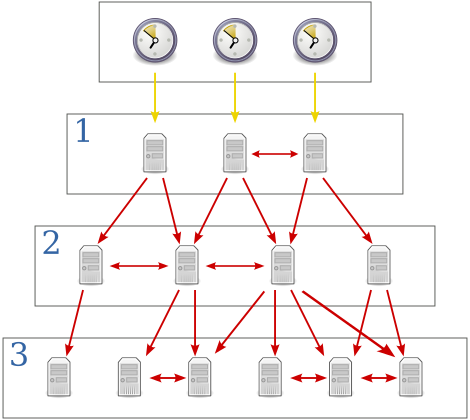
\includegraphics[width=0.7\linewidth]{imagenes/ntp_tree}
	\caption[Esquema de una red de distribución de tiempo usando NTP.]{En este 
	diagrama se 
	muestra una posible red de distribución de tiempo usando NTP. En el estrato 
	0 se hayan las fuentes de reloj de alta estabilidad como GPSDO o relojes 
	atómicos. Estas se conectan directamente a los servidores del estrato 1 que 
	forman los llamados servidores de tiempo primarios. Esta capa provee la 
	hora UTC al resto de los niveles. Como se puede ver se pueden establecer 
	enlaces entre equipos del mismo nivel, además, pueden estar conectados a 
	varios servidores de la capa superior (redundancia). Imagen tomada de 
	\cite{website:imgNTPtree}}
	\label{fig:ntptree}
\end{figure}


El límite superior para un estrato es el 15. Para indicar que un dispositivo no 
está sincronizado se utiliza el valor de estrato 16. El algoritmo \gls{ntp} 
está diseñado para construir una topología con los caminos más cortos hacía los 
servidores del estrato 1 (haciendo uso del algoritmo Bellman-Ford) lo que 
minimiza el tiempo de ida y vuelta acumulado entre los servidores de estrato 1 
y los clientes. A continuación se describen brevemente los estratos más 
relevantes:

\begin{itemize}
	\item \textbf{Estrato 0} \\ A este nivel se encuentran las fuentes de 
	tiempo de alta precisión, entre las que cabe destacar los relojes atómicos 
	o los osciladores disciplinados por GPS (\acrshort{gpsdo}). Generan una 
	señal de un pulso por segundo (\acrshort{pps}) que permite disciplinar el 
	oscilador interno del servidor conectado a la fuente de nivel 0.
	
	\item \textbf{Estrato 1} \\ Lo forman los servidores cuyos relojes se 
	disciplinan directamente con la señal recibida de una fuente de nivel 0 
	logrando una sincronización en torno a unos pocos microsegundos. Además 
	pueden conectarse con otros del mismo nivel para tareas de comprobación de 
	errores o para redundancia.
	
	\item \textbf{Estrato 2 (en adelante)} \\ Los dispositivos de cada estrato 
	se 
	sincronizan con el estrato anterior, pudiendo hacerlo con varios servidores 
	a la vez, y además pueden hacerlo con otros computadores del mismo nivel a 
	fin de mejorar la calidad del servicio.
\end{itemize}

\subsection{Algoritmo}

La figura \ref{fig:ntptree} muestra un esquema de organización típico para una 
red de distribución de tiempo usando \gls{ntp}. Para realizar el cálculo del 
desfase del reloj cliente con respecto al servidor, se emplean una serie de 
paquetes con marcas de tiempo (\textit{timestamps}). El cliente debe iniciar el 
proceso realizando una petición al servidor como muestra la figura 
\ref{fig:ntpts}. El servidor recibe el paquete y lo sella en el instante $T_i$. 
Para realizar los cálculos se emplean siempre las 4 marcas más recientes. Con 
ello se puede realizar el cálculo del tiempo de ida y vuelta ($\delta_i$), y el 
desfase del reloj ($theta_i$) del cliente con respecto al del sevidor en el 
instante de tiempo $T_i$:

\begin{equation}\label{ntprtt}
	\delta_i = (T_{i-2}-T_{i-3}) - (T_{i-1}-T_{i})
\end{equation}\label{ntpoffset}
\begin{equation}
	\theta_i = \frac{(T_{i-2}-T_{i-3}) + (T_{i-1}-T_{i})} {2}
\end{equation}

Hay que tener en cuenta que el servidor no tiene por qué contestar a las 
peticiones del cliente de forma inmediata. El proceso encargado de la gestión 
del servicio \gls{ntp} puede ser interrumpido por otra tarea con más prioridad, 
lo que hace que el tratamiento de las marcas de tiempo no sea determinista.

\begin{figure}
	\centering
	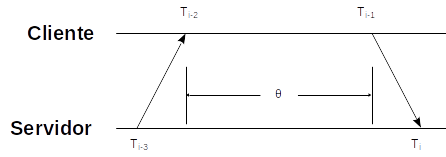
\includegraphics[width=0.7\linewidth]{imagenes/ntp_ts}
	\caption[Cálculo del desfase entre cliente y servidor]{La figura muestra un 
	intercambio de paquetes con marcas de tiempo entre cliente y servidor. Para 
	calcular el tiempo de ida y vuelta se utilizan 4 marcas de tiempo.}
	\label{fig:ntpts}
\end{figure}

\subsection{Rendimiento}

Al ser \gls{ntp} un protocolo que se implementa completamente en 
\textit{software}, no se consigue una gestión determinista para el cálculo del 
desfase entre las dos entidades que se sincronizan. Ello conlleva una 
limitación severa a la exactitud alcanzable mediante el uso de este protocolo 
\incomment{Mejorar esa frase}. Aunque este hecho podría ser tratado mediante el 
uso de sistemas operativos de tiempo real o técnicas que consigan reducir la 
latencia con la que el proceso encargado de la gestión del protocolo \gls{ntp} 
es ejecutado, existe otro factor de diseño que tiene incluso más peso en la 
precisión alcanzable por éste: la asunción de igualdad entre los caminos de ida 
y vuelta para los paquetes enviados por la red de comunicación. En \gls{ntp} se 
considera que el camino de transmisión de los paquetes es simétrico al camino 
de recepción, lo cual es bastante improbable en redes conmutadas con varios 
saltos y múltiples caminos como es el caso de Internet. Todo ello conlleva que 
la exactitud que alcanza este protocolo de forma general, sincronizando dos 
equipos, se sitúe en el orden de los milisegundos llegando a decenas de 
microsegundos en condiciones controladas.
\section{Precision time protocol}

Aunque el desarrollo del protocolo \gls{ntp} supuso un gran avance con respecto 
a las técnicas de sincronización en redes utilizadas anteriormente, la 
exactitud que podía alcanzar dicho protocolo no era suficiente para las 
aplicaciones con requisitos de altas prestaciones como los sistemas de control 
o sistemas de medición distribuidos. Para mejorar el rendimiento se propuso el 
desarrollo de un protocolo denominado \acrlong{ptp}, bajo el estándar 
\acrshort{ieee} 1588-2002 (año de su publicación) \cite{IEEE1588-2008}. 
Actualmente se utiliza la segunda revisión del estándar: IEEE 1588-2008 o 
\gls{ptp}v2, que no presenta compatibilidad con la versión anterior.

\subsection{Arquitectura de red}

El protocolo \gls{ptp} define una arquitectura jerárquica de tipo 
maestro-esclavo. Al igual que en la red \gls{ntp}, en la raíz se sitúa una 
fuente de tiempo muy estable que se conecta al nodo raíz denominado 
\textit{GrandMaster}. Los nodos intermedios pueden actuar como maestros del 
nivel siguiente o como nodos finales. Se definen 5 tipos básicos de 
dispositivos \gls{ptp}, de forma resumida:

\begin{itemize}	
	\item \textbf{\acrfull{oc}} \\
	Este tipo de nodos se comunican con el resto de la red via una única 
	intefaz de red física de tipo bidireccional que se encarga del intercambio 
	de los paquetes con las marcas de tiempo con el resto de la red. La 
	configuración de \gls{oc} sólo permite una única ejecución del protocolo 
	\gls{ptp} y un único estado de funcionamiento. Así, este tipo de 
	configuración, permite al dispositivo actuar como maestro de la red 
	(\gls{gm}) o como reloj esclavo.
	
	\item \textbf{\acrfull{bc}} \\
	Los dispositivos que actúan como \gls{bc} suelen disponer de múltiples 
	puertos físicos que pueden actuar como si fuesen \gls{oc}s pero que 
	comparten una misma referencia de tiempo (recuperada del nodo maestro en el 
	nivel superior). Es decir, uno de los puertos se configurará como esclavo y 
	el resto podrán actuar como puertos maestros para los siguientes nodos de 
	la red.
	
	\item \textbf{\acrfull{tc}} \\
	La gran diferencia con respecto a los tipos anteriores reside en que los 
	\gls{tc} no se sincronizan con un nodo maestro. Estos actúan como simples 
	repetidores del tráfico entrante, pero modifican el campo de corrección de 
	los mensajes \textit{Follow\_UP o Pdelay\_Resp\_Follow\_UP} para incluir el 
	tiempo de residencia de los paquetes \gls{ptp} en el \gls{tc}. El campo de 
	corrección es usado posteriormente por los \gls{oc} para realizar el ajuste 
	de su reloj interno. 
	Existen dos tipos de \glossary{tc}:
	\begin{itemize}
		\item \textit{End-to-end}
		\item \textit{Peer-to-peer}
	\end{itemize}
\end{itemize}

\subsection{Algoritmo}

En el protocolo \gls{ptp} se distinguen dos fases en la ejecución normal:
\begin{enumerate}
	\item Establecimiento de la jerarquía en la red.
	\item Sincronización de los relojes.
\end{enumerate}

\incomment{a ver donde pongo esto...}

Los mensajes \gls{ptp} se pueden clasificar dentro de dos clases: mensajes de 
evento y mensajes generales. Todos los mensajes de tipo evento son sellados 
temporalmente tanto en el momento de la emisión como en el de la recepción. 
Dicha marca temporal indica el momento en el que un paquete abandona o ingresa 
en un nodo y entra o sale del medio de transmisión. Con ello se obtienen las 4 
marcas de tiempo necesarias en el cálculo del tiempo de propagación y del 
desfase entre relojes. El intercambio de mensajes típico se muestra en la 
Figura \ref{fig:ptpts}.


\begin{itemize}
	
	\item \textbf{Sync} \\
	Es un mensaje transmitido de maestro a esclavo que permite medir el retardo 
	de propagación para un paquete en dicho sentido de comunicación. Para ello 
	se sella temporalmente el paquete al ser enviado por el maestro y se 
	acompaña dicha marca de tiempo al paquete (o se envía en otro paquete 
	posterior de tipo \textit{Follow\_Up}) para que el nodo esclavo pueda 
	realizar los cálculos. Estos paquetes proporcionan las marcas temporales 
	$T_1 y T_2$.
	
	\item \textbf{Delay\_Req} \\
	Este mensaje lo sella temporalmente el nodo esclavo y lo envía al maestro 
	para obtener la marca temporal de recepción en otro paquete de respuesta 
	denominado \textit{Delay\_Resp}, obteniendo así las marcas $T_3 y T_4$, que 
	junto a las dos anteriores permiten calcular el tiempo de ida y vuelta, y a 
	partir de este el desfase de los relojes.
\end{itemize}

Además de estos tipos existen mensajes especiales para el modo 
\textit{peer-to-peer}. Dado que actualmente el protoclo \gls{wr} solo 
implementa comunicación \textit{end-to-end} se omite la explicación de los 
mismos, que puede ser consultada en \cite{IEEE1588-2008}.

\begin{figure}
	\centering
	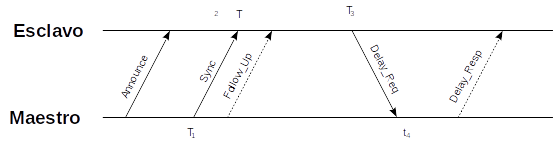
\includegraphics[width=0.7\linewidth]{imagenes/ptp_ts}
	\caption[Intercambio de mensajes para el algoritmo de \acrshort{ptp}]{La 
	figura muestra la secuencia de intercambio de mensajes 
	que se emplea en el algoritmo de \gls{ptp} para conseguir las 4 marcas de 
	tiempo necesarias en el cálculo del \textit{round-trip time} y del desfase.}
	\label{fig:ptpts}
\end{figure}

Para la clase de mensajes generales caben ser destacados los siguientes:

\begin{itemize}
	\item \textbf{Announce} \\
	Es el tipo de mensaje utilizado para informar al resto de los nodos acerca 
	del nodo que transmite (estado y características) además de quién es su 
	\gls{gm}. Son utilizados por el algoritmo \gls{bmc}.
	
	\item \textbf{Follow\_Up} \\
	Sirve para transmitir la marca de tiempo en la escala del maestro para la 
	emisión del mensaje \textit{Sync}.
	
	\item \textbf{Delay\_Resp} \\
	Análogo al anterior para el caso del mensaje \textit{Delay\_Req}.
	
	\item \textbf{Gestión y señalización} \\
	Se engloban mensajes para control y gestión de los relojes o para 
	transmitir información general de estado entre los nodos.
	
\end{itemize}

\incomment{hasta aquí}

En el arranque del algoritmo \gls{ptp} se espera por un lapso de tiempo a 
recibir mensajes de tipo \textit{Announce} provenientes de algún maestro en la 
red. Si no se reciben mensajes de ese tipo, el nodo asume que es maestro hasta 
que un maestro con mejores prestaciones aparezca en la red.

La fase de sincronización se basa en el intercambio de una serie de paquetes 
con marcas de tiempo que permiten al nodo esclavo el cálculo del desfase de su 
reloj con respecto al de referencia en el nodo maestro. El proceso se describe 
en la Figura \ref{fig:ptpts}:

\begin{enumerate}
	\item El maestro manda un mensaje \textit{Sync} \incomment{mejorar 
	redacción} al esclavo con la marca de tiempo $T_1$.
	
	\item El esclavo anota el tiempo de recepción (en su propia escala de 
	tiempo) del mensaje en la marca $T_2$.
	
	\item Dependiendo del soporte \textit{hardware} presente en el maestro la 
	marca $T_1$ puede estar incluida dentro del paquete del \textit{Sync} o 
	necesitar del envío de otro paquete de tipo \textit{Follow\_Up}.
	
	\item El esclavo manda un mensaje de tipo \textit{Delay\_Req} al maestro y 
	almacena la marca de tiempo en que lo hace ($T_3$).
	
	\item El maestro sella la recepción del paquete recibido y la envía dentro 
	de un paquete de tipo \textit{Delay\_Resp}.
\end{enumerate}

Como en el caso de \gls{ntp}, se considera que el tiempo de propagación de los 
mensajes en el camino de ida es igual al de vuelta. En un escenario realista 
esto no tiene por qué complirse. Por tanto, cualquier asimetría existente 
introduce un error en el cómputo del valor de desfase.

\incomment{por la p.108}



\subsection{Rendimiento}

Como se ha visto la esencia del mecanismo de sincronización de \gls{ptp} es 
similar al visto anteriormente en la sección de \gls{ntp}: se intercambian una 
serie de paquetes con marcas de tiempo entre dos nodos de la red para calcular 
el desfase entre sus relojes, entonces ¿cómo se consigue la mejora? La gran 
diferencia entre ambos protocolos es la inclusión en el primero del sellado de 
tiempo a nivel de \textit{hardware}. Cuando un paquete de tipo \gls{ptp} llega 
a un puerto, este genera un evento para que una lógica especial realice un 
sellado de tiempo de dicho paquete. Dicha lógica se encuentra entre la capa 
física (PHY) y la capa de enlace (MAC) del modelo \acrshort{osi} 
(\textit{\acrlong{osi}}).




\section{White Rabbit}

\acrfull{wr} hace referencia tanto al protocolo diseñado como mejora de 
\gls{ptp}v2 como al proyecto internacional que se encarga de su desarrollo y 
mantenimiento. Inicialmente parte como una tecnología desarrollada por el 
\gls{cern} para actualizar el sistema de sincronización y envío de datos de 
control para su complejo de aceleradores de partículas. Gracias a el espíritu 
abierto con el que se desarrolló la tecnología (y a su prometedor rendimiento) 
fueron sumándose otras instituciones al desarrollo, tanto desde el ámbito 
académico, donde cabe destacar el Centro de Investigación de Iones Pesados 
(\textit{Gesellschaft für Schwerionenforschung}, GSI en alemán) en Alemania o 
la propia Universidad de Granada; como desde el empresarial, donde se está 
intentando expandir la tecnología al ámbito industrial. Ejemplos de ello son la 
empresa Seven Solutions (\text{spin-off} de la UGR) en Granada, o CreoTECH en 
Polonia. 

Aunque el empuje en el ámbito de la ciencia es mucho más 
evidente gracias a la inclusión de \textit{WR} en instalaciones para 
aceleradores de partículas, institutos metrológicos o en sistemas de 
adquisición ditribuida como el caso del proyecto Square Kilometre Array (SKA) 
que se está contruyendo en Sudáfrica y que una vez concluido será el 
instrumento de observación astronómica más sensible jamás construido por la 
humanidad. En el caso de la empresa privada, \gls{wr} se ve todavía como una 
tecnología muy prometedora para diversas áreas como Smart Grid, 
Geo-posicionamiento o para las telecomunicaciones, que aún necesita madurar. 
Esto está a punto de cambiar gracias a su inclusión en la próxima revisión del 
estándar \gls{ptp} bajo un nuevo perfil de alta precisión.

Los objetivos de desarrollo iniciales estaban enfocados al entorno de los 
aceleradores de partículas, priorizando una sincronización de calidad junto a 
un sistema que fuese determinista y fácil de mantener:

\begin{itemize}
	\item Lograr para una red de miles de nodos, conectados por enlaces de 
	fibra óptica de hasta 10 km, una diferencia menor del nanosegundo entre dos 
	nodos cualesquiera de la red, es decir, una exactitud de sincronización 
	\textbf{sub-nanosegundo}. Además, se requiere una precisión en el orden del 
	picosegundo.
	
	\item Permitir que el enlace utilizado para los paquetes del protocolo 
	\gls{wr} se pueda \textbf{compartir para} el envío de \textbf{datos de 
	propósito general}, 
	reduciéndo así costes en el despliegue de las infraestructuras.
	
	\item Realizar un desarrollo \textbf{simple y escalable} que no necesite de 
	sofisticados procedimientos de configuración o calibración.
	
	\item Establecer un envío \textbf{determinista} para los paquetes 
	prioritarios, con 
	retardos que no superen ciertos valores umbrales. Esto es especialmente 
	importante en sistemas de control donde la respuesta a un evento no puede 
	exceder un tiempo límite en su envío.
	
	\item Proveer un \textbf{diseño} de referencia \textbf{abierto} a la 
	comunidad 
	(tanto \textit{hardware} como \textit{software}) para fomentar el 
	desarrollo por parte de esta, y evitar las ligaduras con fabricantes.
\end{itemize}

En la actualidad se puede afirmar que en su mayor parte se han cumplido dichos 
objetivos. El requisito principal de rendimiento es algo que se ha conseguido 
en su mayor parte aunque hace falta aportar datos acerca del comportamiento del 
protocolo en redes realmente grandes con un gran número de nodos. La tendencia 
actual en cuanto a rendimiento se centra en la mejora de la exactitud alcanzada 
en escenarios no tan típicos, como enlaces de larga distancia o escenarios con 
cambios en las condiciones de operación. También se investiga como reducir el 
ruido producido por los componentes del sistema de sincronización para lograr 
una precisión en el orden del femtosegundo. El envío determinista es algo que 
no siempre se logra, ya que se puede producir la pérdida de algún paquete de 
alta prioridad en casos de congestión del enlace. Las herramientas de gestión y 
mantenimiento es otro punto al que todavía le queda trabajo por delante y al 
que se está prestando bastante atención dado que son algo crucial si se 
pretende extender el uso del protocolo más allá del ámbito científico.

El protocolo \gls{wr} fue diseñado como una extensión del protocolo IEEE 
1588-2008 (\gls{ptp}v2) al que se añadieron varias mejoras como un modelo de 
enlace más preciso, técnicas de calibración automática o sintonización de los 
relojes mediante el envío de la frecuencia maestra codificada en los paquetes 
transmitidos.




%\chapter{Conclusión y trabajo futuro}
%\input{referencias}
%\addcontentsline{toc}{chapter}{Blibiografía}
%
%
%

%%\chapter{Conclusiones y Trabajos Futuros}
%
%\backmatter
%%\nocite{*}
\addcontentsline{toc}{chapter}{Bibliografía}
\bibliographystyle{plain}
\bibliography{bibliografia/wr_bib}


\appendix
%\input{apendices/manual_usuario/manual_usuario}
%%\input{apendices/paper/paper}
%\input{glosario/entradas_glosario}
\addcontentsline{toc}{chapter}{Lista de Acrónimos}
\printglossaries

\thispagestyle{empty}

\end{document}
